%!TEX root = ../main.tex

\newcommand{\ggT}{\texttt{ggT}}

\chapter{Algebra und Zahlentheorie}
\begin{definition}{Halbgruppe}
	
\end{definition}
\begin{definition}{Monoid}
	
\end{definition}
\begin{definition}{Gruppe}
	
\end{definition}
\begin{definition}{Ring}
	
\end{definition}
\begin{definition}{Körper}
	
\end{definition}
\begin{definition}{Homomorphismus}
	
\end{definition}



\begin{definition}{Gruppe}
	
\end{definition}


Größter gemeinsamer Teiler
\begin{lstlisting}
function ggt(m,n)
begin
	if m = 0 then 
		return n
	else 
		return ggT(n mod m, m)
	end if
end
\end{lstlisting}




\chapter{Diskrete Wahrscheinlichkeit}
\section{Kombinatorik}





%!TEX root = ../main.tex
\chapter{Modulare Arithmetik}
Wir rechnen in den sogenannten Restklassen. Für ein $n\in\N$ seien für $k\in\Z$ die Mengen
\begin{equation*}
	k+n\Z=\simpleset{\ldots,k-2n,k-n,k,k+n,k+2n,\ldots}.
\end{equation*}
die sogenannten Restklassen. Wir definieren hierauf die Äquivalenzrelation $\equiv (\operatorname{mod} n)$ durch
\begin{equation*}
	k\equiv l\mod n\Leftrightarrow k\in l+n\Z
\end{equation*}
Aus den Restklassen bilden wir den Restklassenring $\Z/n\Z$ mit den Verknüpfungen
\begin{align*}
	(k+n\Z)+(l+n\Z)&=k+l+n\Z\\
	(k+n\Z)*(l+n\Z)&=k*l+n\Z\\
\end{align*}
Die multiplikative Gruppe in $\Z/n\Z$ besteht aus den bezüglich Multiplikation invertierbaren Elementen. Sie wird bezeichnet mit $(\Z/n\Z)^\ast$.

Wir bezeichnen mit $\varphi(n)$ die Anzahl der natürlichen Zahlen $k<n$ für die $\ggT(k,n)=1$ gilt. Die multiplikative Gruppe $(\Z/n\Z)^\ast$ hat also $\varphi(n)$ viele Elemente.


\section{Wichtige Sätze und Lemmas}
\begin{itemize}
	\item Allgemein gilt
	\begin{equation*}
		\ggT(ca,cb)=c*\ggT(a,b)
	\end{equation*}
	\item \textbf{Lemma von Bezout}
	Für alle $m,n\in\Z$ existieren $a,b\in\Z$ so, dass
	\begin{equation*}
		\ggT(m,n)=am+bn
	\end{equation*}
	das heißt, der größte gemeinsame Teiler lässt sich als Linearkombination darstellen.
	\item \textbf{Fundamentalsatz der Arithmetik} Sei $n\in\N$. Dann lässt sich $n$ eindeutig darstellen als
	\begin{equation*}
		n=\prod_{p\text{ Prim}}  p^{n_p}
	\end{equation*}
	Dabei ist $n_p\neq 0$ genau dann, wenn $p$ ein Teiler von $n$ ist. Das heißt also, die Primfaktorzerlegung einer Zahl ist eindeutig.
	\item Die multiplikative Gruppe besteht aus den Elementen, die teilerfremd zum Modul sind
	\begin{equation*}
		(\Z/n\Z)^\ast =\set{k+n\Z}{\ggT(k,n)=1}
	\end{equation*}
	\item $\Z/n\Z$ ist ein Körper genau dann, wenn $n$ eine Primzahl ist.

	\item Die lineare Abbildung $x\mapsto kx$ auf $\Z/n\Z$ ist genau dann bijektiv, wenn $\ggT(k,n)=1$.
	
	\item Sind $m,n$ teilerfremd, d.h. $\ggT(m,n)=1$, dann ist
	\begin{equation*}
		\pi:\Z\rightarrow\Z/m\Z\times\Z/n\Z, x\mapsto(x+m\Z,x+n\Z)
	\end{equation*}
	surjektiv. Damit erhält man eine bijektive Abbildung
	\begin{equation*}
		(x\mod mn)\mapsto (x\mod m,x\mod n)
	\end{equation*}
	\item \textbf{Chinesischer Restsatz}
	Für teilerfremde Zahlen $m,n$ ist die Abbildung
	\begin{equation*}
		\Z/mn\Z\rightarrow \Z/m\Z\times \Z/n\Z
		x+mn\Z\mapsto (x+m\Z,x+n\Z)
	\end{equation*}
	ein Isomorphismus (bijektiver Homomorphismus).

	\item \textbf{Der kleine Satz von Fermat} Für alle Primzahlen $p$ und alle $a\in\Z$ gilt
	\begin{equation*}
		a^p\equiv a\mod p
	\end{equation*}
	Falls $a$ und $p$ teilerfremd sind, gilt sogar
	\begin{equation*}
		a^{p-1}\equiv 1\mod p
	\end{equation*}

	\item \textbf{Satz von Euler} Für teilerfremde ganze Zahlen $a,n$ gilt
	\begin{equation*}
		a^{\varphi(n)}\equiv 1 \mod n
	\end{equation*}

	dies gilt sogar für jede kommutative Gruppe $G$ und jedes $a\in G$ (die multiplikative Gruppe $(Z/n\Z)^\ast$ ist kommutativ)
	\begin{equation*}
	 	a^{|G|}=1
	\end{equation*} 

	\item Summe über die $\phi(t)$ der Teiler von $n$ ist gleich $n$
	\begin{equation*}
		\sum_{t|n}\varphi(t)=n
	\end{equation*}
\end{itemize}


\section{Beispiele und Anwendungen}
\subsection{Lösen von Kongruenzen}
\subsubsection{Finden der Inversen in der multiplikativen Gruppe}
Das Finden des Inversen eines Elements in der multiplikativen Gruppe $(\Z/n\Z)^\ast$ efolgt durch Lösen einer besonderen linearen diophantischen Gleichung. Wollen wir das Inverse von $a$ bestimmen, so wollen wir die Kongruenz
\begin{equation*}
	a*x\equiv 1 \mod n
\end{equation*}
für $x$ lösen. Das Inverse existiert nur, wenn $a$ und $n$ teilerfremd sind, das heißt $\ggT(a,n)=1$ ist. Damit lässt sich das Problem auf die diophantische Gleichung
\begin{equation*}
	a*x+n*y = 1 = \ggT(a,n)
\end{equation*}
reduzieren. Wir wissen aus dem Lemma von Bezout, dass sich der $\ggT$ als Linearkombination darstellen lässt. Diese können wir mit dem erweiterten euklidischen Algorithmus finden.
\paragraph{Beispiel:}
Wir wollen das Inverse von $17$ in $(\Z/31\Z)^\ast$ bestimmen. Wir wissen, dass $\ggT(17,31)=1$, wir wollen also folgendes lösen
\begin{align*}
	&17*x\equiv 1 \mod 31\\
	&17*x+31*y=1=\ggT(17,31)
\end{align*}
Dafür führen wir den euklidischen Algorithmus durch, der $\ggT$ ist markiert
\begin{align*}
	31&=1*17+14\\
	17&=1*14+3\\
	14&=4*3+2\\
	3&=1*2+\fbox{1} \leftarrow \text{ ab hier nach oben arbeiten.}\\
	2&=2*\fbox{1}+0.
\end{align*}
Gehen wir nun aus der vorletzten Zeile die Schritte rückwärts zurück, erhalten wir
\begin{align*}
	1&=3-2\\
	&=3-(14-4*3)=5*3-14\\
	&=5*(17-14)-14=5*17-6*14\\
	1&=5*17-6*(31-17)=\fbox{11}*17-6*31
\end{align*}
womit wir bereits die Linearfaktorzerlegung und damit insbesondere das Inverse gefunden haben.

\subsubsection{Lösen einer allgemeinen diophantischen Gleichung}
Möchte man eine lineare diophantische Gleichung 
\begin{equation*}
	a*x+b*y=c
\end{equation*}
lösen bei der $c\neq\ggT(a,b)$ ist, muss man wie folgt vorgehen.

Zu erst ist wichtig, dass $c$ ein Vielfaches von $\ggT(a,b)$ sein muss, sonst ist die Gleichung nicht lösbar.

Dann kann man wie oben vorgehen, den $\ggT$ berechnen und anschließend die vorletzte Zeile so erweitern, dass der Rest gleich $c$ ist. Verfährt man nun weiter wie oben und setzt rückwärts ein, erhält man die gesuchte Lösung.

\subsection{Fehlererkennung}


\subsection{Primzahltest und -Zertifikat}
\subsubsection{Primzahltest nach Fermat 22.3}

\subsubsection{Exaktes Primzahlzertifikat}
Sei $n\geq 2$ und $n\in\N$. Falls für alle Primzahlen $p$ mit $n\equiv 1\mod p$ eine Zahl $a\in Z$ existiert, so dass
\begin{equation*}
 	a^{n-1}\equiv 1\mod n \text{\quad und \quad}a^{\frac{n-1}p}\not\equiv 1\mod n
\end{equation*}
gilt, dann ist $n$ eine Primzahl. 

\subsection{Simultane Kongruenzen lösen}
\subsection{Schnelle Exponentiation 22.6}
\subsection{RSA}
Das RSA-Verfahren ist ein asymmetrisches Verschlüsselungsverfahren, das sehr weit verbreitet ist.

Möchte Bob  ($B$) eine Nachricht an Alice ($A$) senden, so muss Alice zunächst das folgende vorbereiten 
\begin{enumerate}
	\item Große Primzahlen $p,q$ mit $p<q$, beide müssen geheim bleiben.
	\item Berechne $n=p*q$ (öffentlich),
	\item setze $\varphi(n)=(p-1)(q-1)$,
	\item wähle $e>1$ mit $\ggT(e,\varphi(n)=1$ (öffentlich), diese Zahl wird zum Verschlüsseln verwendet.
	\item Berechne $s<n$ mit $e*s\equiv 1\mod \varphi(n)$, d.h. $e*s=k*\varphi(n)+1$. Diese Zahl wird zum Entschlüsseln verwendet und muss unbedingt geheim bleiben.
\end{enumerate}
Das Paar $(n,e)$ bildet den \emph{öffentlichen Schlüssel}.

Bobs Nachricht muss im Bereich $\simpleset{0,\ldots,n-1}$ sein, dies kann zum Beispiel durch Aufteilen der Nachricht in mehrere Teile erreicht werden. Die Nachricht sei $x$.

Bob verschlüsselt nun
\begin{equation*}
	y=x^e\mod n
\end{equation*}

Alice kann dann wieder entschlüsseln mit
\begin{equation*}
	x'=y^s\mod n
\end{equation*}

Dies funktionert, da
\begin{align*}
	(x^e)^s = x^{e*s}=x^{k*\varphi(n)+1}=x*(x^{\varphi(n)})^k\equiv x*1^k\mod n
\end{align*}
%!TEX root = ../main.tex
\chapter{Graphen}
Wir beschränken uns auf einfache ungerichtete Graphen.
\begin{definition}{Einfacher ungerichteter Graph}
	Ein \emph{einfacher ungerichteter Graph} ist ein Paar $(V,E)$ wobei $V$ die Menge der Knoten und $E\subseteq \binom V2$ die Menge der Kanten ist.
\end{definition}

\begin{definition}{Komplementgraph}
	Für einen Graph $G=(V,E)$ ist der \emph{Komplementgraph} der Graph $G'=\left(V,\binom V2\setminus E\right)$.
\end{definition}

\begin{definition}{Isomorphie}
	Zwei Graphen $G_1=(V_1,E_1)$ und $G_2=(V_2,E_2)$ sind \emph{isomorph}, falls es eine bijektive Abbildung $\varphi:V_1\rightarrow V_2$ gibt, so dass für alle $u,v\in V_1$ gilt:
	\begin{equation*}
		\simpleset{u,v}\in E_1\Leftrightarrow \simpleset{\varphi(u),\varphi(v)}\in E_2
	\end{equation*}
\end{definition}

\begin{definition}{Bipartiter Graph}
	Wenn die Knotenmenge $V$ des Graphen $G=(V,E)$ so in zwei Teile $V_1,V_2$ aufgeteilt werden kann, dass für jede Kante $\simpleset{u,v}\in E$ genau einer der beiden Knoten in $V_1$ und der andere in $V_2$ liegt, so spricht man von einem \emph{bipartiten Graphen}.
\end{definition}

Da eine Kante nach Definition eine zweielementige Menge ist, kann man für eine Kante $e$ und einen Knoten $v$ ob $v\in e$ gilt. Wir sagen dann $u$ und $e$ sind \emph{inzident}.

Zwei Knoten sind adjazent (benachbart), wenn es eine Kante zwischen ihnen gibt, d.h. $\simpleset{u,v}\in E$ bedeutet, dass $u$ und $v$ adjazent sind.

Der Grad des Knotens $u\in V$ ist die Anzahl der Kanten die zu $u$ inzident sind.

\begin{definition}{Weg}
	Ein Weg (auch Pfad) in einem Graph $(V,E)$ ist eine Folge von Knoten $(v_0,\ldots,v_n)$ von Knoten $v_i\in V$ mit der Eigenschaft, dass für alle $1\leq i\leq n$ gilt
	\begin{equation*}
	 	\simpleset{v_{i-1},v_i}\in E
	\end{equation*}
	Die Länge des Weges ist $n$, man zählt also die Anzahl durchlaufener Kanten.

	In einem einfachen Weg sind alle Knoten verschieden. 
\end{definition}
Ein Weg heißt Eulerweg, wenn auf ihm jede Kante des Graphen genau einmal durchlaufen wird.


\begin{definition}{Kreis}
	Ein Kreis ist ein Pfad, bei dem Start- und Endknoten gleich sind.

	In einem einfachen Kreis sind alle Knoten außer der erste und letzte verschieden.
\end{definition}
Ein Eulerweg der gleichzeitig ein Kreis ist, heißt Eulerkreis.

\begin{definition}{Planarität}
	Ein Graph heißt planar, wenn er sich so in die Ebene einzechnen lässt, dass sich die Kanten nicht schneiden.
\end{definition}

Eine Facette ist eine zusammenhängende Fläche, die von Kanten berandet ist, insbesondere ist das Äußere immer eine Facette.

\section{Sätze zu Graphen}
\begin{itemize}
	\item Die Summe aller Knotengrade in einem ungerichteten Graphen ist immer gerade.
	\item In jedem endlichen Graph ist die Anzahl der Knoten mit ungeradem Grad gerade.
	\item Ein zusammenhängender endlicher Graph hat genau dann einen Eulerpfad, wenn die Anzahl der Knoten mit ungeradem Grad maximal 2 ist. Ein Eulerkreis existiert genau dann, wenn alle Knoten geraden Grad haben.
	\item \textbf{Eulerformel} In endlichen zusammenhängenden planaren Graphen mit $n\geq 1$ Knoten, $m$ Kanten und $f$ Facetten gilt
	\begin{equation*}
		n-m+f=2\text{\quad bezeihungsweise\quad}n-m+f=z+1
	\end{equation*}
	für $z$ Zusammenhangskomponenten.
	Wichtige Folgerungen hieraus sind
	\begin{itemize}
		\item Ein planarer Graph mit $n\geq 3$ Knoten hat höchstens $3n-6$ Kanten.
		\item Ein planarer bipartiter Graph mit $n\geq 4$ Knoten hat höchstens $2n-4$ Kanten
		\item In jedem planaren Graph gibt es mindestens einen Knoten mit Grad kleiner oder gleich $5$.
		\item Der $K_5$ und der $K_{3,3}$ sind nicht planar.
	\end{itemize}

	\item \textbf{Satz von Kuratowski} Ein Graph ist genau dann planar, wenn er keine Unterteilung des $K_5$ oder des $K_{3,3}$ enthält.
\end{itemize}

\section{Wichtige Graphen und deren Eigenschaften}
\begin{itemize}
	\item Der $K_4$ ist der vollständige Graph mit 4 Knoten

	\begin{center}
		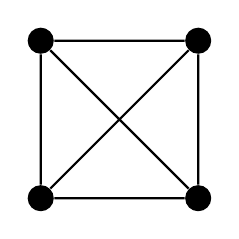
\begin{tikzpicture}
			\draw node[circle, fill=black, minimum width=4pt] (1) at (0,0) {};
			\draw node[circle, fill=black, minimum width=4pt] (2) at (2,0) {};
			\draw node[circle, fill=black, minimum width=4pt] (3) at (0,2) {};
			\draw node[circle, fill=black, minimum width=4pt] (4) at (2,2) {};

			\draw[thick] (1) -- (2) -- (3) -- (4) -- (1) -- (3) -- (4) -- (2);
		\end{tikzpicture}
	\end{center}

	Im $K_n$ haben alle Knoten den Grad $n-1$. Die Graphen $K_2=P_2,K_3=C_3$ und $K_4$ sind planar, der $K_5$ jedoch nicht.

	\item Der $P_5$ ist der Pfad-Graph mit 5 Knoten

	\begin{center}
		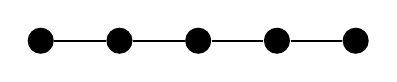
\begin{tikzpicture}
			\draw node[circle, fill=black, minimum width=4pt] (1) at (0,0) {};
			\draw node[circle, fill=black, minimum width=4pt] (2) at (1,0) {};
			\draw node[circle, fill=black, minimum width=4pt] (3) at (2,0) {};
			\draw node[circle, fill=black, minimum width=4pt] (4) at (3,0) {};
			\draw node[circle, fill=black, minimum width=4pt] (5) at (4,0) {};

			\draw[thick] (1) -- (2) -- (3) -- (4) -- (5);
		\end{tikzpicture}
	\end{center}

	Der $P_n$ hat für $n\geq 2$ immer einen Eulerweg aber keinen Eulerkreis. Alle $P_n$ sind planar.

	\item Der $C_6$ ist der Kreis-Graph mit 6 Knoten
	\begin{center}
		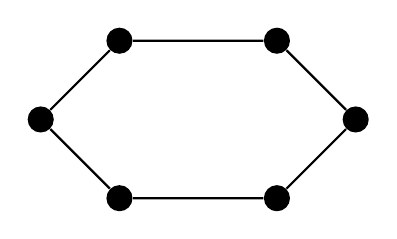
\begin{tikzpicture}
			\draw node[circle, fill=black, minimum width=4pt] (1) at (0,0) {};
			\draw node[circle, fill=black, minimum width=4pt] (2) at (2,0) {};
			\draw node[circle, fill=black, minimum width=4pt] (3) at (3,1) {};
			\draw node[circle, fill=black, minimum width=4pt] (4) at (2,2) {};
			\draw node[circle, fill=black, minimum width=4pt] (5) at (0,2) {};
			\draw node[circle, fill=black, minimum width=4pt] (6) at (-1,1) {};

			\draw[thick] (1) -- (2) -- (3) -- (4) -- (5) -- (6) -- (1);
		\end{tikzpicture}
	\end{center}

	Der kleinste Kreis-Graph ist der $C_3$.

	Der $C_n$ hat immer einen Eulerkreis. 

	Alle $C_n$ sind planar.

	Im $C_n$ hat jeder Knoten hat den Grad 2. 

	\item Der $K_{3,3}$ ist der bipartite Graph mit jeweils 3 Knoten in einer Partition

	\begin{center}
		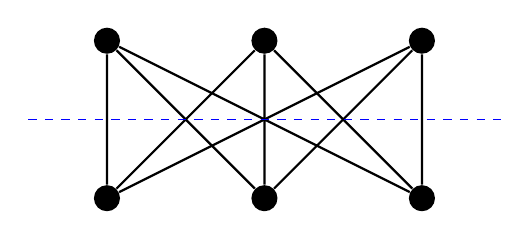
\begin{tikzpicture}
			\draw node[circle, fill=black, minimum width=4pt] (1) at (0,2) {};
			\draw node[circle, fill=black, minimum width=4pt] (2) at (2,2) {};
			\draw node[circle, fill=black, minimum width=4pt] (3) at (4,2) {};
			\draw node[circle, fill=black, minimum width=4pt] (4) at (0,0) {};
			\draw node[circle, fill=black, minimum width=4pt] (5) at (2,0) {};
			\draw node[circle, fill=black, minimum width=4pt] (6) at (4,0) {};

			\draw[thick] (1) -- (4) -- (2) -- (5) -- (1) -- (6) -- (3) -- (5);
			\draw[thick] (4) -- (3);
			\draw[thick] (2) -- (6);

			\draw[blue, dashed] (-1,1) -- (5,1);
		\end{tikzpicture}
	\end{center}

	Im $K_{3,3}$ hat jeder Knoten den Grad $3$.

	Der $K_{3,3}$ ist nicht planar.
\end{itemize}
%!TEX root = ../main.tex
\chapter{Wichtige Abschätzungen}

\section{Wachstum der Fakultät}
\begin{equation*}
	\log(n!)\in \Theta(n\log n)
\end{equation*}
denn es gilt 
\begin{align*}
	\forall n\geq 2:\quad \left(\frac n2\right)^{\frac n2} < n! < n^n \text{ oder auch } e*\left(\frac ne\right)^n\leq n!\leq n*e*\left(\frac ne\right)^n
\end{align*}

\section{Wachstum des Binomialkoeffizienten}
Wir interessieren uns für die Binomialkoeffizienten der Form $\binom{2n}{n}$ bzw. $\binom{n}{\lceil \frac n2\rceil}=\binom{n}{\lfloor \frac n2\rfloor}$ (diese sind die Binomialkoeffizienten mit größtem Wert) für große $n$.
Aus dem binomischen Lehrsatz folgt (mit $a=b=1$), dass
\begin{equation*}
	\sum_k\binom nk = 2^n.
\end{equation*}
Damit wissen wir, dass die Binomialkoeffizienten im Durchschnitt von der Größenordnung $\frac{2^n}n$ sind. Damit folgt
\begin{equation*}
	\forall n\geq 3:\quad\binom{n}{\lceil \frac n2\rceil}=\binom{n}{\lfloor \frac n2\rfloor}>\frac{2^n}n
\end{equation*}



\section{Wachstum des kleinsten gemeinsamen Vielfachen}
\newcommand{\kgV}{\texttt{kgV}}
Wir definieren zunächst
\begin{equation*}
	\kgV(n)=\kgV(2,\ldots,n).
\end{equation*}
es ist also das kleinste gemeinsame Vielfache der ersten $n$ natürlichen Zahlen.

\section{Fibonacci-Zahlen}
\begin{equation*}
	F_0 = 0, F_1=1, F_n=F_{n-1}+F_{n-2}\enspace\forall n\geq 2
\end{equation*}

Sogenannte Dominostein-Interpretation der Fibonacci-Zahlen:
Es stehen beliebig viele Dominosteine von zwei Sorten zu Verfügung, solche der Länge 1 und solche der Länge 2.

Wie viele Möglichkeiten gibt es, damit eine Sequenz der Länge $n$ zu legen? $\rightsquigarrow F_n$

\subsection{Abschätzung der Fibonacci-Zahlen}
Es gilt 
\begin{align*}
	&F_n\leq 2^n\leq F_{2n}\\
	\text{bzw. }&2^n\leq F_{2n}\leq 2^{2n}\\
	\text{bzw. }&(\sqrt 2)^n\leq F_n\leq 2^n
\end{align*}
dies lässt sich durch Induktion leicht zeigen.

Es gilt
\begin{equation*}
	\ggT(F_m,F_n)=F_{\ggT(m,n)}.
\end{equation*}



\section{Catalanzahlen}

